% Chapter 3

\chapter{Análisis y diseño}
\label{capitulo3}

\section{Análisis}
La resolución de los problemas siempre debe empezar con un análisis acerca de su alcance y características. El análisis surge con las ideas de soluciones del problema para en base a ellas diseñar una resolución del mismo. Para la fase de análisis se ha realizado un Documento de Visión (Apéndice \ref{visionDoc}) y una Especificación de Requerimientos (Apéndice \ref{ersDoc}).

\subsection{Visión}
El resto del documento de visión se puede encontrar en el Apéndice \ref{visionDoc}. Aquí se ha incluido la parte de mayor consideración.

\subsubsection{Propósito}
Ayudar a mejorar los métodos de enseñanza que ofrece la Universidad Técnica Particular de Loja en cuanto a la programación y uso de base de datos para las carreras de Sistemas y Electrónica.

\subsubsection{Alcance}
\index{Editar Código} \index{Persistir Código} \index{Calificar Código} \index{Controlar Versiones de Código} \index{Ejecutar Código} \index{Sincronizar Notas por LTI} \index{Autenticación LTI}
Se propone un sistema de editar código en línea que a su vez integra LMS \index{LMS} externos (para autenticación y notas), un servidor de control de versiones externo (para la persistencia de código), y un servicio web de ejecución de código en línea de una forma segura, eficaz y eficiente (para dar un ambiente de ejecución y pruebas tanto para los usuarios del sistema como para calificar de una forma automática).

\subsubsection{Oportunidad de Negocio}
Con el avance continuo de la tecnología y su introducción en varios aspectos de la vida cotidiana, hay una necesidad creciente de ingenieros en sistemas e electrónica que puedan programar y entender el software funcional en adición a las bases de datos que están por detrás de estos mismos sistemas.

\index{Editar Código}
Por la razon antes mencionada, está de moda ofrecer plataformas en línea para la enseñanza dinámica de la programación. GitEDU espera ofrecer las mismas funcionalidades a un costo institucional menor a través de integración con sistemas existentes e innovación para proveer una mejor experiencia de usuario, tanto estudiantes como profesores para llevarse a cabo un mejor proceso de aprendizaje.

\subsubsection{Demográfia del mercado}
En el año 2011, la Universidad Técnica Particular de Loja contaba con aproximadamente 4000 estudiantes presenciales y 24000 estudiantes a distancia con una tendencia creciente \citep{UTPL-Datos-Estadisticos}. En la experiencia personal del autor, las carreras de Sistemas y Electrónica, por lo menos en la modalidad presencial, juntas representan aproximadamente un 10\% de todos los estudiantes en la universidad, lo cual daría aproximadamente un mínimo 2800 estudiantes afectados por un nuevo sistema. Según el directorio de docentes de la universidad, son 60 profesores en el departamento de Ciencias de la Computación y Electrónica \citep{UTPL-Directorio-Docentes}. Con eso se puede estimar un mínimo de 2860 usuarios que el sistema propuesto podría llegar a afectar.

Es precisamente la parte de la población y de usuarios potenciales mencionados anteriormente, que están involcrados en el proceso de enseñar, evaluar y aprender habilidades de programación/consulta a bases de datos, que forman la base de usuarios de la aplicación.

\subsection{Especificacion de Requerimientos}
El resto del documento de especificación de requerimientos se puede encontrar en el Apéndice \ref{ersDoc}. A continuación se ha incluido las partes mas importantes.

\subsubsection{Propósito}
El siguiente documento espera dar una descripción detallada de los requisitos del Sistema Git Education (GitEDU) con la finalidad de definir la intención de la misma, declarar de forma completa todos los componentes a ser desarrollados del sistema, y también explicar limitaciones del mismo además de sus interacciones e interfaces con otros sistemas. Se destina el siguiente documento para revisión por el equipo de asesores y como una referencia de alcance para el equipo de desarrollo.

\subsubsection{Alcance}
GitEDU es un sistema de integración para promover la programación estudiantil y el sistema educativo que soporta el mismo. El sistema final debe disponer de buena documentación y alta calidad de código para sostener su futuro desarrollo y mantenimiento por parte de una comunidad de profesionales y profesionales en formación.

\index{Editar Código} \index{Persistir Código} \index{Calificar Código} \index{Controlar Versiones de Código} \index{Ejecutar Código} \index{Autenticación LTI} \index{Sincronizar Notas por LTI}
Docentes de las carreras involucrados en la enseñanza de programación, tanto en la carrera de Sistemas Informáticos y Computación como en la carrera de Electrónica y Telecomunicaciones, actualmente pueden agergar en la plataforma, deberes, talleres, pruebas y exámenes, donde a través de los LMS \index{LMS} institucionales pueden compartir los mismos con sus alumnos. Los alumnos pueden entrar a través de un enlace que su docente comparta dentro del LMS \index{LMS} institucional y con un canal de comunicación LTI\index{LTI}, la plataforma GitEDU les identifica y autentica sin interacción del usuario para que el estudiante pueda empezar directamente con el trabajo que tiene que realizar sin digitar sus credenciales. En el curso de su actividad, se va guardando su progreso periódicamente contra un servidor de control de versiones institucional (GitLab CE) y en cualquier momento el estudiante puede probar e interactuar con su código a través de un terminal virtual de Linux que se encuentra dentro de la misma interfaz. Una vez que termina su trabajo y desee enviarlo, se lo envía y el código escrito se auto califica contra un conjunto de pruebas unitarias ocultas que el docente agregó a la actividad al crearlo. La nota que se genera se lo envía al LMS \index{LMS} institucional a través del mismo canal LTI\index{LTI}. En caso de que el docente decide no utilizar pruebas unitarias o calificar cada trabajo a mano o realizar una calificación híbrida entre las pruebas unitarias y la parte a mano, no se reflejarán las notas en el LMS \index{LMS} hasta que el docente haya terminado de calificar el código en la plataforma de GitEDU.

\subsubsection{Perspectiva de Producto}
\index{Editar Código} \index{Persistir Código} \index{Calificar Código} \index{Controlar Versiones de Código} \index{Ejecutar Código}
La plataforma GitEDU se compone de dos subsistemas: el subsistema de editar código y el subsistema de ejecutar código. El subsistema de editar código consiste en la integración de autenticación y notas por el lado del LMS, el uso de persistencia del código por el servidor de control de versiones por otro lado, el consumo de un servicio de ejecución de código por un tercer lado y un editor de código en línea. El subsistema de ejecutar código consiste en esperar llamadas del subsistema anterior, validar la autenticidad, establecer permisos, limitaciones y parámetros de ejecución, gestionar recursos para ejecución, la ejecución interactiva y devolución de resultados al otro subsistema.

Debido a la necesidad de mantener la seguridad y prevenir la ejecución indebida de código, el subsistema debe ser aislado de todos los usuarios y solo accedido desde el otro subsistema a través de un API que permite su interoperabilidad. La solución para la ejecución de código debe ser liviana debido al gran número de usuarios concurrentes que se pueda tener a la vez.

\subsubsection{Funcionalidades de Producto}
\index{Editar Código} \index{Persistir Código} \index{Calificar Código} \index{Controlar Versiones de Código} \index{Ejecutar Código} \index{Autenticación LTI}
Para entrar al subsistema de editar código en línea, se debe autenticar contra el LMS \index{LMS} institucional. El editor de código en línea debe soportar una gran variedad de lenguajes y estar abierto a la agregación de más lenguajes en un futuro. La persistencia de código en un servidor de control de versiones debe ser transparente y no requerir ningún interacción del usuario. La interfaz para interactuar con el ambiente virtual debe ser simple y fácil de manejar sin mayor conocimiento de las tecnologías que le respaldan. Se debe poder acompañar al editor de código con documentación que guíe al estudiante en explicar o resolver el problema actual. La manera en que los docentes pueden generar nuevos ejercicios, su documentación y pruebas unitarias para la calificación debe ser intuitivo.

\subsubsection{Características de usuario}
Los tres tipos de usuarios que interactúan con el sistema son Docentes, Alumnos y Administradores. Cada tipo de usuario tiene sus propias necesidades y requerimientos.

\index{Editar Código} \index{Persistir Código} \index{Calificar Código} \index{Controlar Versiones de Código} \index{Ejecutar Código}
Docentes, necesitan un sistema que sea fácil de manejar y que simplifique y automatice el proceso de enseñar y evaluar a los estudiantes. Eso significa tener una interfaz intuitiva para los docentes puedan escribir, documentar y generar pruebas unitarias para probar la funcionalidad de código que escriben los estudiantes para los ejercicios.

\index{Editar Código} \index{Ejecutar Código}
Alumnos, necesitan un sistema que les brinde una buena experiencia de aprendizaje y les proporcione todas las herramientas que requieren para programar en línea. al igual que sus profesores, los elumnos deben disponer de una interfaz intuitiva que les ayude a cumplir con las responsabilidades de estudiar, aprender y demostrar conocimientos en una cantidad de tiempo óptimo.

Administradores, necesitan un sistema que sea seguro y cuyos componentes sean fáciles de mantener y extender a lo largo del tiempo. Para ello se necesita tener una buena documentación del funcionamiento del sistema y todos sus componentes para tener la misma como referencia.

\subsubsection{Limitaciones}
\index{Ejecutar Código}
Se requiere de hardware con alta capacidad de virtualización y conectividad al internet y la intranet institucional para poder brindar la mejor experiencia al usuario.

\subsubsection{Suposiciones y Dependencias}
Se supone que siempre habrá la conectividad necesaria para poder usar todos los componentes del sistema.

\subsubsection{División de Requerimientos}
En caso de que falte recursos de tiempo o algún otro recurso, se limitará el alcance del proyecto para enfocarse en los requerimientos de prioridad más alta y dejar los demás requerimientos para trabajos futuros.

\section{Diseño}
Previo a la implementación de cualquier sistema es importante analizar su funcionamiento y en base a esto realizar un diseño que provee de las funcionalidades que se requiere. Por lo tanto, a continuación se demuestra las fases del diseño realizado desde la definición de sistemas, subsistemas y módulos así como la interacción entre ellos, hasta la arquitectura interna y de despliegue.

\subsection{Sistemas, Subsistemas y Módulos}
\index{Editar Código} \index{Persistir Código} \index{Calificar Código} \index{Controlar Versiones de Código} \index{Ejecutar Código} \index{Autenticación LTI} \index{Sincronizar Notas por LTI}
Debido a la naturaleza del alcance de este trabajo de titulación, se considera que se debe dividir la plataforma en dos sistemas que sean capaces de interactuar entre sí. El primer sistema es el que ofrece el editor de código en línea, integración con los LMS \index{LMS} institucionales y a su vez integración con un servidor de control de versiones. El segundo sistema solo se encarga de ejecución de código en línea a través de algún tipo de virtualización y aislamiento de procesos. De esta forma se puede aislar el sistema que está bajo mayor riesgo de ser atacado (el de ejecución de código arbitrariamente) del sistema con mayor riesgo de impacto negativo (el sistema de escribir código en línea, el cual también se encarga de las calificaciones). A continuación se presenta la interacción entre los sistemas y actores en el Diagrama de Contexto de Sistemas.

\begin{landscape}

	% figure 
	\begin{figure}
	  \begin{center}
	    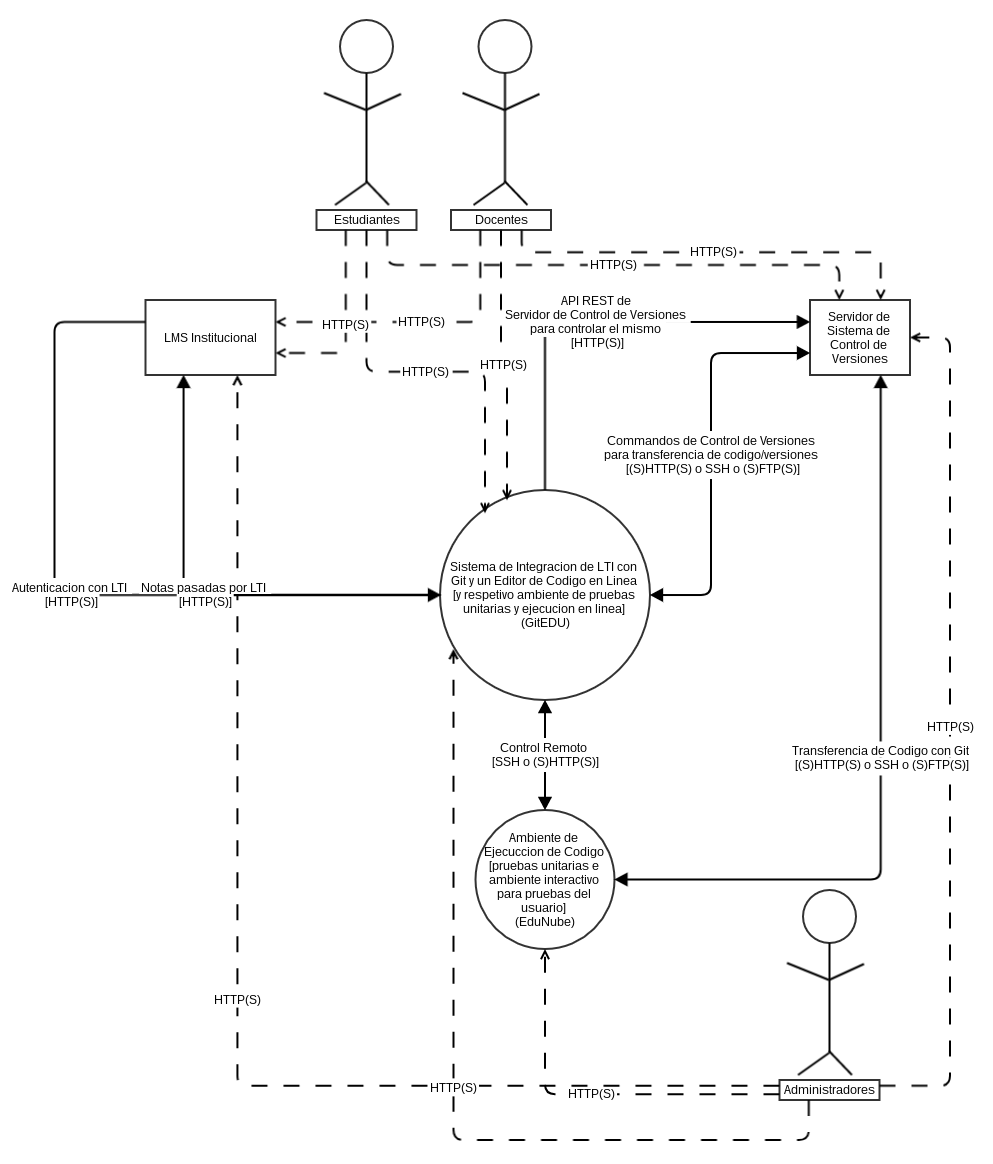
\includegraphics[width=1.7\textwidth]{Figures/contexto.png}
	  \end{center}
	  \caption{Diagrama de Contexto para GitEdu y EduNube.}
	  \label{context}
	\end{figure}

\end{landscape}

El diagrama de contexto visualizado en la figura \ref{context} demuestra la relación entre las tres clases de usuario, sistemas existentes, los sistemas que se plantea desarrollar y los protocolos de interacción entre sistemas distintos y también entre humanos y sistemas.

\index{Editar Código} \index{Persistir Código} \index{Calificar Código} \index{Controlar Versiones de Código} \index{Ejecutar Código} \index{Autenticación LTI} \index{Sincronizar Notas por LTI}
Los tres tipos de usuarios que se considera para el sistema son administradores, quienes administran y mantienen todo el sistema en su ambiente de despliegue; docentes, quienes generan contenido didáctico para sus estudiantes y califican los mismos motivo por el cual tienen acceso a los LMS, el sistema de editar codigo (que les permite generar nuevas tareas / exámenes / pruebas / talleres para sus estudiantes y ver el progreso y calificaciones de los mismos) y el sistema de control de versiones (donde puede ver y bajar código que escriben los estudiantes y ver a un nivel más profundo el historial y evolución del mismo), y estudiantes, quienes tienen acceso a los mismos tres sistemas que tienen los docentes. Los estudiantes acceden al LMS \index{LMS} donde ven las tareas / exámenes / pruebas / talleres nuevos que hay y al abrirlos les lleva a identificase y autenticarse en el sistema de editar código en línea mediante LTI\index{LTI}. Los estudiantes realizan sus tareas de código, mientras que los datos se respaldan de forma automática en un servidor de control de versiones independiente de tal forma que lo pueden revisar tanto los estudiantes involucrados como su docente a futuro. Aquel control adicional podría llegar a ser una evidencia importante para la resolución de conflictos entre estudiantes y/o docentes a futuro.

\index{Editar Código} \index{Persistir Código} \index{Calificar Código} \index{Controlar Versiones de Código} \index{Ejecutar Código} \index{Autenticación LTI} \index{Sincronizar Notas por LTI}
El sistema de editar codigo, que en este documento se conoce simplemente bajo el nombre GitEDU, controla remotamente por medio de comandos, y una mezcla de protocolos (SSH, HTTP sobre SSH [SHTTP] y HTTPS), dependiendo de cómo sea el caso, un sistema de ejecucion de código, conocido a partir de aquí en adelante como EduNube, señala acciones que debe tomar el segundo y/o datos que necesita sincronizar con el primer sistema. Al mismo tiempo, GitEDU comunica con el servidor de control de versiones mediante su API externa (una API REST) sobre HTTP o HTTPS para controlar el mismo y prepararle para flujos continuos de código editado que puede viajar por una variedad de protocolos como SHTTP, HTTPS, HTTP, SFTP, FTP o FTPS como requiera la situación y ambiente de despliegue. Cuando EduNube requiere de codigo de algún usuario para realizar una calificación o algún otro tipo de interacción con un usuario que requiere probar el mismo, primero se procede a descargar el código involucrado desde el servidor de control de versiones sobre uno de los protocolos mencionado previamente para el mismo. En base a la naturaleza de las operaciones que se está haciendo, comunica sus resultados con GitEDU para que pueda manejar las mismas de la forma adecuada. En el caso de notas, GitEDU se encarga de sincronizar las mismas con los LMS \index{LMS} institucionales con los cuales está integrado mediante el protocolo LTI\index{LTI}.

\pagebreak

\begin{landscape}

	% figure
	\begin{figure}
	  \begin{center}
	    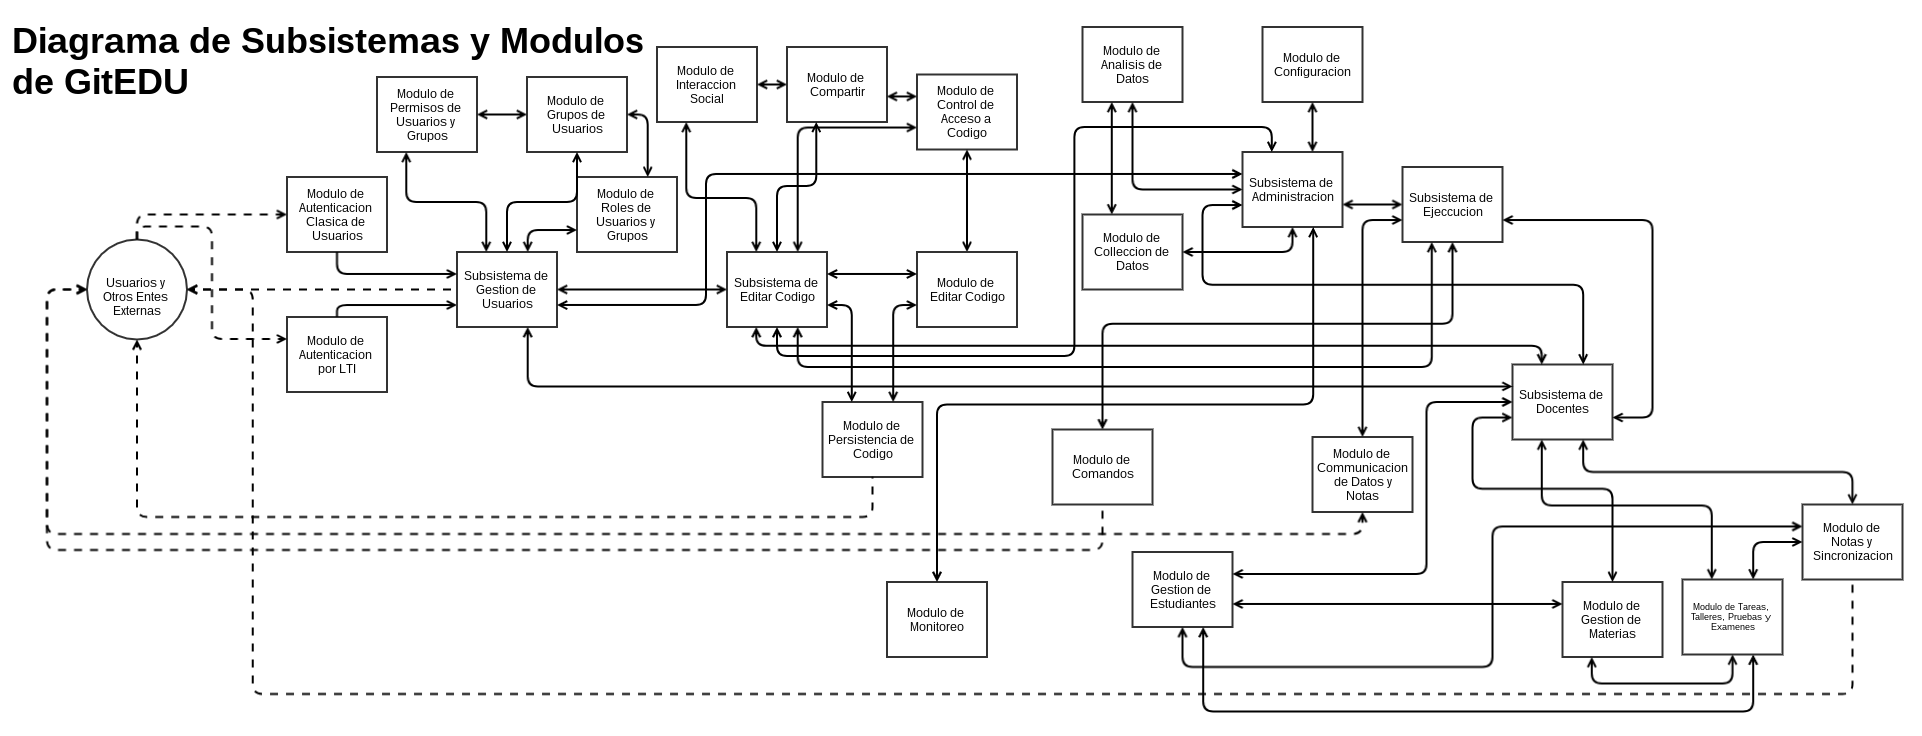
\includegraphics[width=1.7\textwidth]{Figures/mod_ge.png}
	  \end{center}
	  \caption{Diagrama de Subsistemas y Módulos de GitEdu.}
	  \label{mod_ge}
	\end{figure}

\end{landscape}

\subsubsection{GitEdu}

La figura \ref{mod_ge} presenta todos los componentes en forma de subsistemas y módulos que forman parte del diseño propuesto para el sistema GitEdu.

\paragraph{Subsistema de Gestión de Usuarios}
\index{Autenticación LTI}
El subsistema de gestión de usuarios se encarga de temas de seguridad y acceso por usuarios a varios componentes de la aplicación. Para esto autentica usuarios mediante dos módulos (uno clásico y el otro mediante el protocolo LTI\index{LTI}) y lleva un sistema de permisos orientado a usuarios, grupos y roles.

\subparagraph{Módulo de Autenticación Clásica de Usuarios}
El módulo de autenticación clásica de usuarios permite que los usuarios finales puedan iniciar sesión mediante un usuario y contraseña.

\subparagraph{Módulo de Autenticación por LTI}
\index{Autenticación LTI}
El módulo de autenticación por LTI \index{LTI} permite que los usuarios finales puedan iniciar su sesión mediante una existente en algún sistema externo que soporta LTI\index{LTI}.

\subparagraph{Módulo de Grupos de Usuarios}
El módulo de grupos de usuarios permite definir grupos específicos de usuarios cuya membresía les cambia el nivel y naturaleza del acceso que tengan en la aplicación.

\subparagraph{Módulo de Permisos de Usuarios y Grupos}
El módulo de permisos de usuarios y grupos, define la naturaleza de acceso que tienen los usuarios autorizados y los grupos a los cuales pertenecen dentro de la aplicación.

\subparagraph{Módulo de Roles de Usuarios y Grupos}
El módulo de roles de usuarios y grupos define las responsabilidades de varios grupos de usuarios y usuarios específicos, en base a los mismos les asigna permisos adecuados tanto para proteger la aplicación contra el uso y acceso indebido y al mismo tiempo permitir a los usuarios poder realizar sus actividades normalmente sin impedimentos.

\paragraph{Subsistema de Editar Código}
\index{Editar Código}
El subsistema de editar código forma el núcleo de la funcionalidad del sistema GitEdu. Esto lo realiza a través de funcionalidades de editar codigo, persistirlo y permitir la interacción adecuada y social entre usuarios.

\subparagraph{Modulo de Editar Codigo}
\index{Editar Código}
El módulo de editar código en línea ofrece funcionalidades básicas de un editor de código (IDE) en línea.

\subparagraph{Módulo de Persistencia de Código}
\index{Persistir Código}
El módulo de persistencia de código, persiste el código versionado en servidores de control de versiones externos. Al momento de necesitar abrir un código anterior cualquiera, recupera el mismo de los servidores de control de versiones externos para que el usuario pueda seguir editando lo mismo.

\subparagraph{Módulo de Control de Acceso de Código}
El módulo de control de acceso de código permite a los usuarios definir y modificar los permisos que tiene su código para controlar la naturaleza del acceso que tienen otros usuarios, grupos y roles.

\subparagraph{Modulo de Compartir}
El módulo de compartir permite compartir el acceso al código con otros usuarios y grupos.

\subparagraph{Módulo de Interacción Social}
El módulo de interacción social permite que los usuarios puedan interactuar en tiempo real mientras editan juntos el código.

\paragraph{Subsistema de Docentes}
\index{Sincronizar Notas por LTI}
El subsistema de docentes ofrece muchas de las funcionalidades que requieren los docentes para llevar exitosamente su materia de programación. Estas funcionalidades incluyen gestión de estudiantes, materias y notas. La gestión de materias y notas también involucra una gestión y calificación de talleres, deberes, pruebas y exámenes. Además por el hecho de que se genera nuevas notas y calificaciones a través de GitEdu, también se encarga de sincronizar notas con otros sistemas externos como los LMS \index{LMS} a través de LTI\index{LTI}.

\subparagraph{Módulo de Gestión de Estudiantes}
El módulo de gestión de estudiantes permite que los docentes puedan ver notas de sus estudiantes. Además de que los estudiantes puedan revisar sus notas. Los administradores como docentes pueden asignar estudiantes a aulas o cambiar o eliminar asignaciones previas.

\subparagraph{Módulo de Gestión de Materias}
El módulo de gestión de materias permite a los docentes y administradores ver estadísticas de una materia, creación de grupos de estudiantes dentro de una materia (por ejemplo para un proyecto grupal) tanto para un docente o para un estudiante, modificar grupos de estudiantes (por ejemplo eliminar un integrante), y asignar talleres, deberes, pruebas o exámenes a un estudiante, grupo o materia. Además dentro de la gestión de materias, docentes se puede establecer el peso de cada taller, deber, prueba y examen para en base a ello calcular los promedios de un estudiante.

\subparagraph{Módulo de Talleres, Deberes, Pruebas y Exámenes}
El módulo de talleres, deberes, pruebas y exámenes permite a los docentes definir nuevos talleres, deberes, pruebas, exámenes, etc y los criterios de evaluación de los mismos. En ello se incluye las pruebas unitarias (si desea calificación automatizada) y documentación que explica lo que hay que hacer al estudiante.

\subparagraph{Módulo de Notas y Sincronización}
\index{Sincronizar Notas por LTI}
El módulo de notas y sincronización gestiona las notas que mantiene GitEdu y se encarga de sincronizar cambios en las mismas. Aunque realiza este trabajo por detrás normalmente, también proporciona una interfaz gráfica para interacción con los docentes respectivos y adecuados. Además por el tema de seguridad e integridad de las notas, se lleva versionado y con un registro preciso de cuando fueron modificados y por quién.

\paragraph{Subsistema de Ejecución de Código}
\index{Ejecutar Código} \index{Calificar Código}
El subsistema de ejecución de código se encarga de comunicar con el sistema externo EduNube con el fin de aprovechar las funcionalidades del mismo y proveer de funcionalidades de ejecución en línea, aplicación de pruebas unitarias y calificación automática de código sin exponer al sistema EduNube a usuarios finales. Para aumentar la seguridad que logra llevar EduNube, GitEdu se comunica con los mismos a través de canales seguros como HTTPS y SSH, utilizando métodos de autenticación orientados a una esquema de llaves públicas y privadas (criptografía asimétrica) para asegurarse de la identidad de ambos previo al envío de comandos y comunicación de datos y notas.

\subparagraph{Módulo de Comandos}
\index{Ejecutar Código} \index{Calificar Código}
El módulo de comandos se encarga de controlar el sistema de EduNube a través de su API externa para indicar al mismo cuando debe bajar, ejecutar o calificar algún código.

\subparagraph{Módulo de Comunicación de Datos y Notas}
\index{Sincronizar Notas por LTI}
El módulo de comunicación de datos y notas permite la sincronización de los mismos cuando sea necesario entre EduNube y GitEdu.

\paragraph{Subsistema de Administración}
El subsistema de administración ayuda a los administradores de GitEdu a recolectar datos acerca del uso del mismo y analizar los datos, además de ser capaces de configurar y monitorear el rendimiento del sistema.

\subparagraph{Módulo de Configuración}
El módulo de configuración permite la configuración en tiempo real del sistema GitEdu, por ejemplo conexiones con sistemas externos y gestión de usuarios.

\subparagraph{Módulo de Monitoreo}
El módulo de monitoreo permite ver en tiempo real el consumo del sistema.

\subparagraph{Módulo de Recolección de Datos}
\index{Recolección de Datos}
El módulo de recolección de datos lleva un registro contínuo del uso del sistema para su revisión y análisis por parte de operadores humanos, para después realizar temas de auditoría como la toma de decisiones estratégicas.

\subparagraph{Módulo de Análisis de Datos}
\index{Toma de Decisiones}
El módulo de análisis de datos proporciona las herramientas necesarias para que un operador humano pueda interpretar los mismos y sacar sus conclusiones.

\pagebreak

\begin{landscape}

	% figure
	\begin{figure}
	  \begin{center}
	    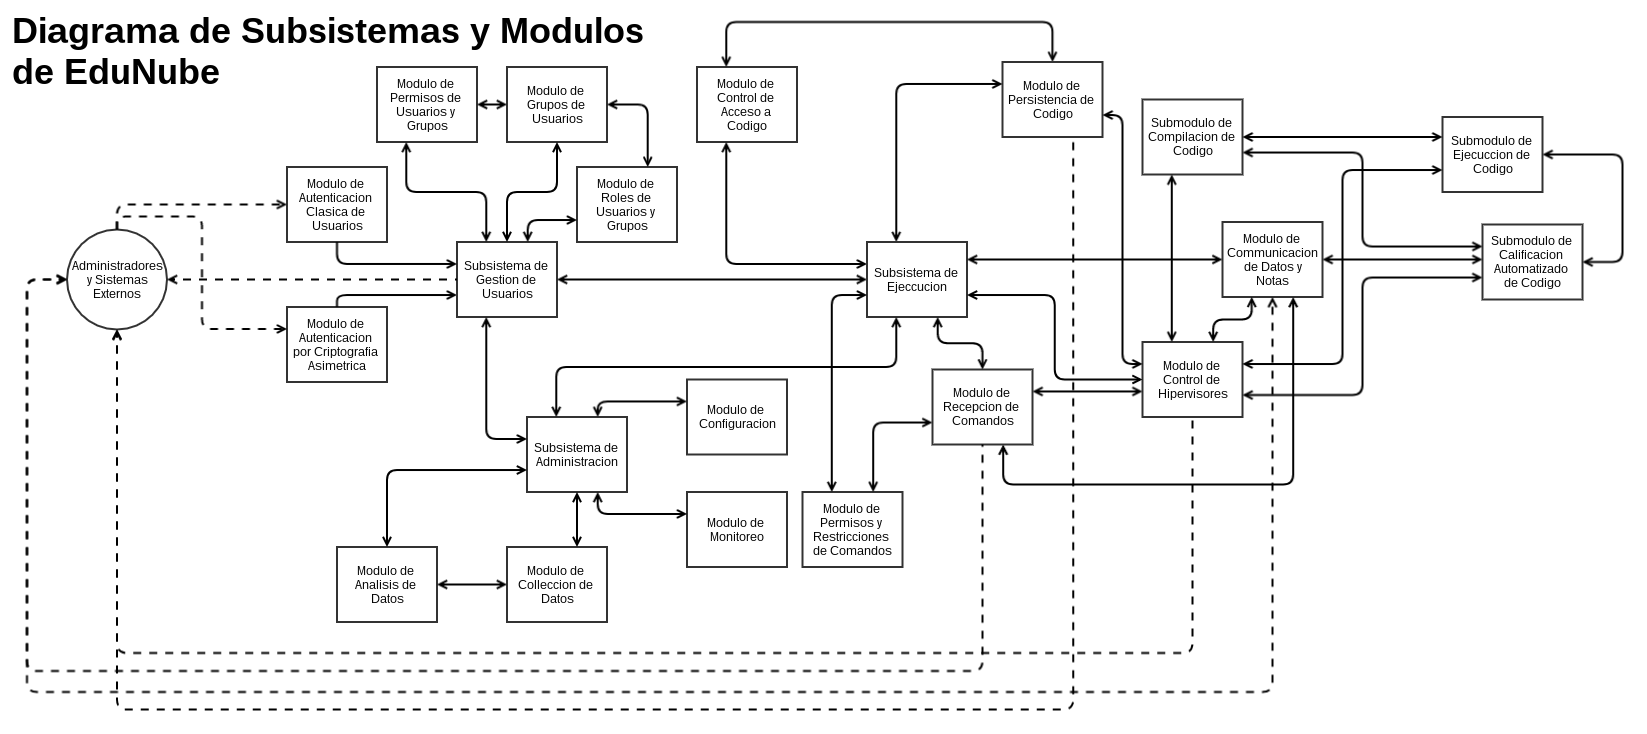
\includegraphics[width=1.7\textwidth]{Figures/mod_en.png}
	  \end{center}
	  \caption{Diagrama de Subsistemas y Módulos de EduNube.}
	  \label{mod_en}
	\end{figure}

\end{landscape}

\subsubsection{EduNube}

La figura \ref{mod_en} presenta todos los componentes en forma de subsistemas y módulos que forman parte del diseño propuesto para el sistema EduNube.

\paragraph{Subsistema de Gestión de Usuarios}
El subsistema de gestión de usuarios de encarga de temas de seguridad y acceso indirecto por usuarios (a través de GitEdu) y acceso directo por parte de administradores a varios componentes de la aplicación. Para lo mismo autentica usuarios mediante dos módulos (uno clásico solo para administración del mismo y el otro mediante llaves públicas/privadas [criptografía asimétrica] para aplicaciones externas) y lleva un sistema de permisos orientado a usuarios, grupos y roles.

\subparagraph{Módulo de Autenticación Clásica de Usuarios}
El módulo de autenticación clásica de usuarios permite que administradores puedan iniciar sesión mediante un usuario y contraseña.

\subparagraph{Módulo de Autenticación por Criptografía Asimétrica}
El módulo de autenticación por criptografía asimétrica permite a los usuarios finales, a través de GitEdu iniciar sesión para la ejecución controlada y remota de comandos y código.

\subparagraph{Módulo de Grupos de Usuarios}
El módulo de grupos de usuarios permite definir grupos específicos de usuarios cuyo membresía les cambia el nivel y naturaleza del acceso que tengan en la aplicación.

\subparagraph{Módulo de Permisos de Usuarios y Grupos}
El módulo de permisos de usuarios y grupos define la naturaleza de acceso que tienen los usuarios autorizados y los grupos a los cuales pertenecen dentro de la aplicación.

\subparagraph{Módulo de Roles de Usuarios y Grupos}
El módulo de roles de usuarios y grupos define las responsabilidades de varios grupos de usuarios y usuarios específicos, en base a esto les asigna permisos adecuados tanto para proteger la aplicación contra uso o accesos indebidos y al mismo tiempo permitir a los usuarios poder realizar sus actividades normalmente sin impedimentos.

\paragraph{Subsistema de Ejecución}
\index{Ejecutar Código} \index{Calificar Código}
El subsistema de ejecución de código se encarga de recibir y procesar  comandos del sistema externo GitEdu con el fin de aprovechar los hipervisores que tiene a su cargo y proveer de las funcionalidades de ejecución en línea, aplicación de pruebas unitarias y calificación automática de código sin exponer dichos hipervisores a usuarios finales. Para aumentar la seguridad que logra llevar EduNube, GitEdu se comunica con lo mismo a través de canales seguros como HTTPS y SSH utilizando métodos de autenticación orientados a un esquema de llaves públicas y privadas (criptografía asimétrica) para asegurar de la identidad de ambos previo al envío de comandos y comunicación de datos y notas.

\subparagraph{Módulo de Recepción de Comandos}
\index{Ejecutar Código} \index{Calificar Código}
El módulo de recepción de comandos se encarga de recibir comandos externos enviados a través del API externa que provee para que otras aplicaciones puedan indicar cuando debe bajar, ejecutar o calificar algún código.

\subparagraph{Módulo de Permisos y Restricciones de Comandos}
\index{Ejecutar Código} \index{Calificar Código}
El módulo de permisos y restricciones de comandos se encarga de limitar o permitir comandos externos recibidos por el sistema EduNube. Se basa en políticas establecidas previamente que definen los horarios de trabajo de ciertos procesos y dependencias de los mismos (por ejemplo no se debe calificar los exámenes de un paralelo hasta que todos terminen). Junto al módulo de control de acceso a código, permite a los docentes y administradores tener control refinado sobre cuando y que está permitido hacer por parte de los usuarios que están usando EduNube a través de GitEdu.

\subparagraph{Módulo de Control de Hipervisores}
\index{Ejecutar Código} \index{Calificar Código}
El módulo de control de hipervisores se encarga de cumplir con funcionalidades críticas del sistema EduNube de compilar, ejecutar y calificar código. Esto lo hace a través de tres respectivos submódulos para cada fase. Este módulo también controla los hipervisores conectados al sistema EduNube con el fin de poder realizar las operaciones listadas previamente.
\begin{description}
	\item[Submódulo de Compilación de Código] \index{Ejecutar Código}
	El submódulo de compilación de código se encarga de compilar código que se entrega en base a procedimientos que define el profesor anteriormente, y reporta resultados del mismo: de éxito o errores de compilación. Para la implementación del mismo submódulo, se aprovecha de las máquinas virtuales que provee el hipervisor con el fin de realizar la compilación en un ambiente controlado y aislado.
    \item[Submódulo de Ejecución de Código] \index{Ejecutar Código}
	El submódulo de ejecución de código recibe de entradas de código compilado y comandos que se desea ejecutar en el ambiente de ejecución y pruebas con el fin de proveer, a través de las máquinas virtuales controladas y aisladas, un ambiente interactivo donde los estudiantes y docentes pueden trabajar de una forma dinámica con código desarrollado dentro de la plataforma.
    \item[Submódulo de Calificación Automatizado de Código] \index{Calificar Código}
	El submódulo de calificación automatizado de código se basa en pruebas unitarias escritas previamente por un docente y que van contra la funcionalidad que se pide en el código de los estudiantes, con el fin de calificar el código de una forma autónoma. Una vez que termina de calificar un código, reporta los resultados a gestores de los mismos.
\end{description}

\subparagraph{Módulo de Persistencia de Código}
\index{Persistir Código}
El módulo de persistencia de código recupera el código versionado en servidores de control de versiones externos que los usuarios han escrito y editado con el fin de permitir la compilación, ejecución y calificación del mismo dentro del sistema EduNube.

\subparagraph{Módulo de Control de Acceso a Código}
\index{Persistir Código}
El módulo de control de acceso a código se encarga de restringir y permitir en base a reglas las operaciones de compilación, ejecución y calificación automatizada de códigos que los usuarios editan. De la misma forma permite definir flujos de trabajo y dependencias para el procesamiento de proyectos en adición a establecer horarios y restricciones de procesamiento para los mismos.

\subparagraph{Módulo de Comunicación de Datos y Notas}
\index{Sincronizar Notas por LTI}
El módulo de comunicación de datos y notas permite la sincronización de los mismos cuando sea necesario entre EduNube y GitEdu.

\paragraph{Subsistema de Administración}
El subsistema de administración ayuda a los administradores de EduNube recolectar datos acerca del uso del mismo y analizarlos, además de ser capaces de configurar y monitorear el rendimiento del sistema.

\subparagraph{Módulo de Configuración}
El módulo de configuración permite la configuración en tiempo real del sistema EduNube, por ejemplo conexiones con sistemas externos, gestión de llaves públicas y privadas, y gestión de usuarios.

\subparagraph{Módulo de Monitoreo}
El módulo de monitoreo permite ver en tiempo real el consumo del sistema y sus hipervisores respectivos.

\subparagraph{Módulo de Recolección de Datos}
\index{Recolección de Datos}
El módulo de recolección de datos lleva un registro contínuo del uso del sistema para su revisión y análisis por parte de los operadores humanos, para después poder hacer temas de auditoría como toma de decisiones estratégicas.

\subparagraph{Módulo de Análisis de Datos}
\index{Toma de Decisiones}
El módulo de análisis de datos proporciona las herramientas necesarias para que un operador humano pueda interpretar los mismos y sacar sus conclusiones.

\subsubsection{Ventajas del Diseño de Sistemas, Subsistemas y Módulos}
La ventaja de un diseño orientado a módulos como se lo presenta aquí es la división de la funcionalidad para ayudar en la extensibilidad y mantenibilidad de los sistemas al largo plazo. Por ejemplo este diseño permite agregar funcionalidad adicional a futuro como autenticación por otros medios (por ejemplo LDAP) o la integración de mecanismos anti-plagio. Esta propiedad puede dar una vida útil mayor a los sistemas desarrollados porque muchas veces no se conoce todo lo que puede requerir un software a futuro para el diseño e implementación inicial. A continuación se presenta la arquitectura de estos dos sistemas, tanto GitEdu como su ambiente de ejecución de código virtualizado, EduNube.

%\begin{itemize}
%	\item \textbf{Seguridad}, auténtica usuarios y controla el acceso que tiene cada uno de ellos. Esto se realiza con los siguientes componentes:
%    \begin{itemize}
%    	\item \textbf{Autenticación por LTI} usa interfaces LTI \index{LTI} de aplicaciones externas como LMS \index{LMS} institucionales para autenticar usuarios.
%		\item \textbf{Autenticación Clásica}, permite el login (autenticación) de usuarios mediante la forma clásica de un usuario y contraseña.
%		\item \textbf{Permisos}, permite otorgar o revocar partes específicas del sistema a usuarios específicos. Ejemplos de permisos podrían ser acceso a la administración de una materia, por ejemplo el control que se da a un docente o grupo de docentes sobre una materia.
%		\item \textbf{Grupos}, permite aplicar el sistema de permisos a grupos de usuarios creados bajo la discreción de usuarios suficientemente privilegiados dentro del sistema. Ejemplos de grupos podrían ser miembros de una cierta materia o tipo de materia, por ejemplo ''Base de Datos''.
%		\item \textbf{Roles}, permite definir usuarios por su propósito del sistema con el fin de aplicarles un conjunto global de permisos asociados por el tipo de usuario que es. Ejemplos de roles podrían ser Estudiante, Docente y Administrador.
%    \end{itemize}
%\end{itemize}

\pagebreak

\begin{landscape}

	% figure
	\begin{figure}
	  \begin{center}
      	% TODO: Bigger? %% AESTHETICS
	    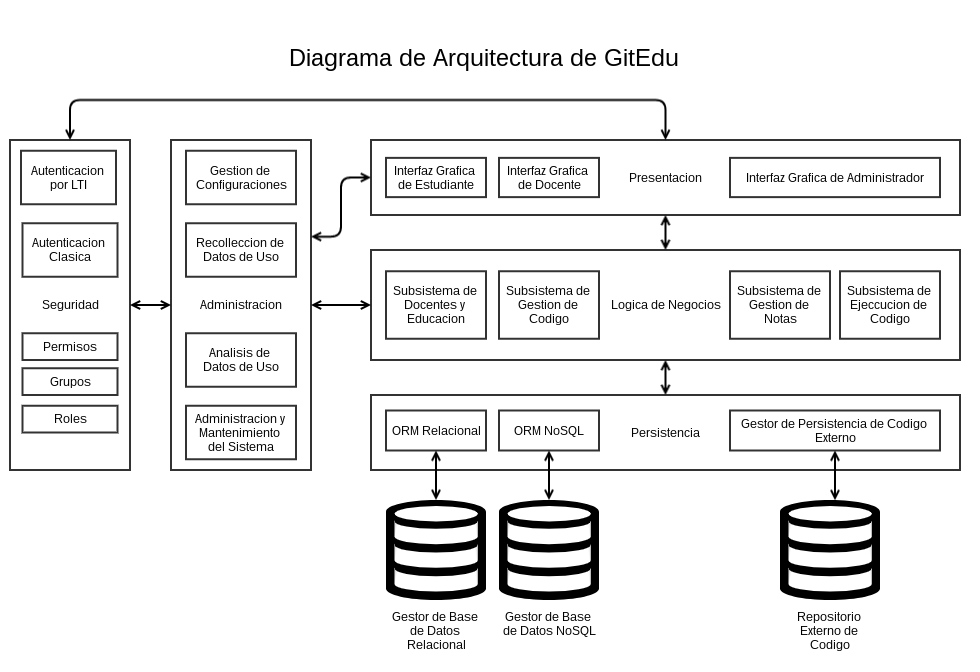
\includegraphics[width=1.0\textwidth]{Figures/arq_ge.png}
	  \end{center}
	  \caption{Diagrama de Arquitectura para el Sistema GitEdu.}
	  \label{arq_ge}
	\end{figure}

\end{landscape}

\subsection{Arquitectura}
Como se puede observar en la figura \ref{arq_ge}, a nivel global, el sistema GitEdu consiste en 5 capas que son:

\begin{itemize}
	\item \textbf{Seguridad}, auténtica usuarios y controla el acceso que tiene cada uno de ellos. Esto se realiza con los siguientes componentes:
    \begin{itemize}
    	\item \textbf{Autenticación por LTI} usa interfaces LTI \index{LTI} de aplicaciones externas como LMS \index{LMS} institucionales para autenticar usuarios. \index{Autenticación LTI}
		\item \textbf{Autenticación Clásica}, permite el login (autenticación) de usuarios mediante la forma clásica, de un usuario y contraseña.
		\item \textbf{Permisos}, permite otorgar o revocar partes específicas del sistema a usuarios específicos. Ejemplos de estos podrían ser: acceso a la administración de una materia, por ejemplo el control que se da a un docente o grupo de docentes sobre una materia.
		\item \textbf{Grupos}, permite aplicar el sistema de permisos a grupos de usuarios creados bajo la discreción de usuarios suficientemente privilegiados dentro del sistema. Ejemplos de estos podrían ser miembros de una cierta materia o tipo de materia, por ejemplo ''Base de Datos''.
		\item \textbf{Roles}, permite definir usuarios por su propósito del sistema con el fin de aplicarles un conjunto global de permisos asociados por el tipo de usuario que es. Ejemplos de roles podrían ser Estudiante, Docente y Administrador.
    \end{itemize}
    \item \textbf{Administración} permite la administración, mantenimiento y recolección de datos por usuarios dentro del sistema. Para cumplir con estas responsabilidades se divide en:
    \begin{itemize}
    	\item \textbf{Subsistema de Gestión de Configuraciones}, que permite a administradores cambiar de forma rápida y fácil las configuraciones internas del sistema.
        \item \textbf{Subsistema de Recolección de Datos de Uso}, que colecta automáticamente datos del uso del sistema. \index{Recolección de Datos}
        \item \textbf{Subsistema de Análisis de Datos de Uso}, que permite a administradores visualizar y analizar los datos que ha recolectado el Subsistema de Recolección de Datos de Uso. \index{Toma de Decisiones}
        \item \textbf{Subsistema de Administración y Mantenimiento}, que permite a administradores ver en tiempo real y también registros históricos de consumo de recursos. Este subsistema también proporciona a administradores las herramientas que necesita para gestionar y controlar problemas como usuarios maliciosos, sistemas caídos entre otros problemas detectados.
    \end{itemize}
    \item \textbf{Presentación}, que se encarga de presentar interfaces web a varias tipos de usuario, incluyendo:
    \begin{itemize}
    	\item \textbf{Estudiantes}
		\item \textbf{Docentes}
		\item \textbf{Administradores}
    \end{itemize}
    \item \textbf{Lógica de Negocios}, que se encarga de llevar a cabo los procesos de negocio para cumplir con el propósito de la aplicación. Esto se subdivide en cuatro subsistemas:
    \begin{itemize}
    	\item \textbf{Subsistema de Docentes y Educación}, que se lleva a cabo procesos de negocio que tienen que ver con enseñanza y evaluación. Dentro de este subsistema también se lleva las tareas de administración asociadas con un docente y sus aulas.
        \item \textbf{Subsistema de Gestión de Código}, lleva el control del código y los procesos asociados. \index{Editar Código}
        \item \textbf{Subsistema de Gestión de Notas}, maneja los procesos de negocio asociados con la sincronización y auditoría de notas generadas dentro del sistema. \index{Sincronizar Notas por LTI}
        \item \textbf{Subsistema de Ejecución de Código}, que lleva a cabo procesos de negocio que tienen que ver con la ejecución arbitraria de código y por lo tanto requiere un cierto nivel de seguridad y aislamiento elevado a través de entornos virtualizados. Dentro de los procesos que se incluyen aquí: compilación, ejecución y calificación de código automatizado mediante pruebas unitarias. \index{Ejecutar Código} \index{Calificar Código}
    \end{itemize}
    \item \textbf{Persistencia}, que se encarga de asegurar que persisten datos importantes para su uso a futuro y también la recuperación de los mismos. Esto se subdivide en tres clases de persistencia:\index{Persistir Código}
    \begin{itemize}
    	\item Persistencia a través de un \textbf{ORM Relacional}, que guarda y recupera datos estructurados de la aplicación en bases de datos relacionales y orienta los mismos datos a objetos dentro de la aplicación para permitir su fácil manipulación.\index{Persistir Código}
        \item Persistencia a través de un \textbf{ORM NoSQL}, que guarda y recupera datos no estructurados de la aplicación en bases de datos no relacionales y orienta los mismos datos a objetos dentro de la aplicación para permitir su facil manipulación.\index{Persistir Código}
        \item Persistencia de código a través de un \textbf{Gestor de Persistencia de Código Externo} que guarda y recupera código de usuarios para su manipulación dentro de la aplicación y persistencia fuera del mismo.\index{Persistir Código}
    \end{itemize}
\end{itemize}

\begin{landscape}
	\begin{figure}
	  \begin{center}
        % TODO: Bigger? %% AESTHETICS
	    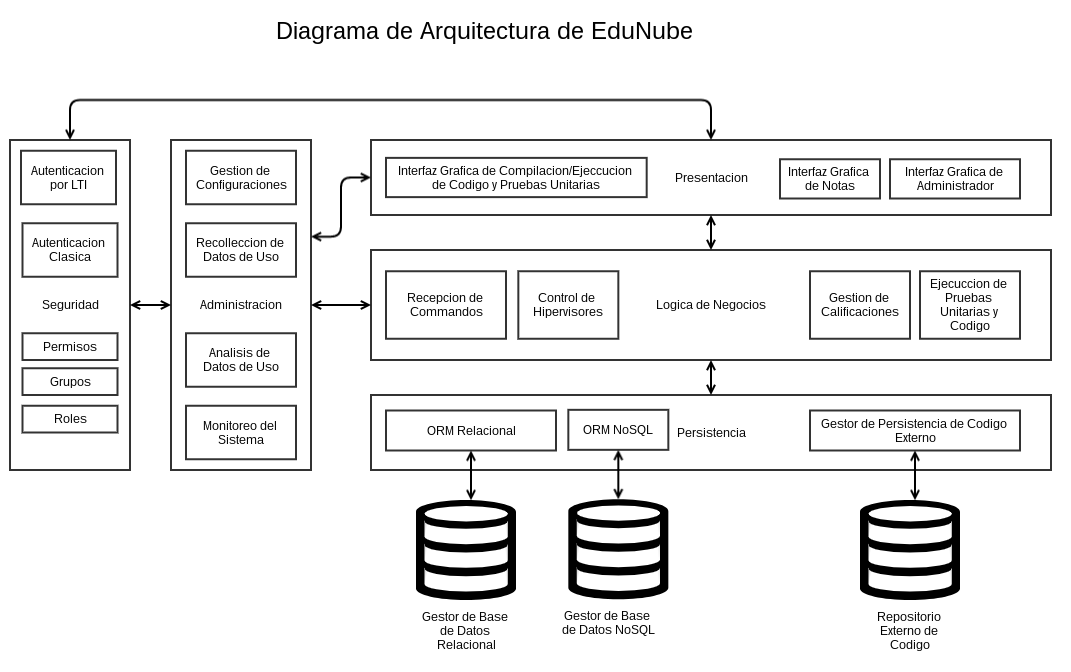
\includegraphics[width=1.0\textwidth]{Figures/arq_en.png}
	  \end{center}
	  \caption{Diagrama de Arquitectura para el Sistema EduNube.}
	  \label{arq_en}
	\end{figure}

\end{landscape}

Como se puede observar en la figura \ref{arq_en}, a un nivel global, el sistema EduNube consiste en 5 capas que son:
\begin{itemize}
	\item \textbf{Seguridad} auténtica administradores y sistemas externos y controla el acceso que tiene cada uno de ellos. Esto se realiza con los siguientes componentes:
    \begin{itemize}
    	\item \textbf{Autenticación por Criptografía Asimétrica}, usa pares de llaves públicas y privadas suficientemente grandes para ser difíciles de falsificar matemáticamente para autenticar sistemas externos.
    	\item \textbf{Autenticación Clásica}, permite el login (autenticación) de administradores mediante la forma clásica de un usuario y contraseña.
    	\item \textbf{Permisos}, permite otorgar o revocar partes específicas del sistema a usuarios específicos. Ejemplos de permisos podrían ser quién puede crear máquinas virtuales o ver el consumo de recursos del sistema.
    	\item \textbf{Grupos}, permite aplicar el sistema de permisos a grupos de usuarios creados bajo la discreción de administradores suficientemente privilegiados dentro del sistema. Ejemplos de estos podrían ser ciertos tipos de usuario que representa algún tipo de estudiante en algún tipo de materia, por ejemplo para la materia de ''Base de Datos''.
    	\item \textbf{Roles}, permite definir usuarios por su propósito en el sistema, con el fin de aplicarles un conjunto global de permisos asociados por el tipo de usuario que es. Ejemplos de roles podrían ser Sistema Externo y Administrador.
    \end{itemize}
	\item \textbf{Administración}, permite la administración, mantenimiento y recolección de datos por usuarios dentro del sistema. Para cumplir con estas responsabilidades se divide en:
    \begin{itemize}
    	\item \textbf{Subsistema de Gestión de Configuraciones}, que permite a administradores cambiar de forma rápida y fácil de las configuraciones internas del sistema.
    	\item \textbf{Subsistema de Recolección de Datos de Uso}, que colecta automáticamente datos del uso del sistema.\index{Recolección de Datos}
    	\item \textbf{Subsistema de Análisis de Datos de Uso}, que permite a administradores visualizar y analizar los datos que ha recolectado el Subsistema de Recolección de Datos de Uso.\index{Toma de Decisiones}
    	\item \textbf{Subsistema de Monitoreo}, que permite a administradores ver en tiempo real y también registros históricos de consumo de recursos. Este subsistema también proporciona a administradores las herramientas que necesita para gestionar y controlar problemas como usuarios maliciosos, sistemas caídos entre otros problemas detectados.\index{Recolección de Datos}\index{Toma de Decisiones}
    \end{itemize}
	\item \textbf{Presentación}, que se encarga de presentar interfaces web a varias tipos de usuario, incluyendo:
    \begin{itemize}
    	\item \textbf{Compilación/Ejecución de Código y Pruebas Unitarias}, proporciona las interfaces gráficas utilizadas durante la compilación y ejecución de código en la aplicación de pruebas unitarias contra un código para ayudar en la calificación del mismo.\index{Ejecutar Código}\index{Calificar Código}
        \item \textbf{Notas}, permite a docentes y sistemas externos ver las notas asignadas a un código.
        \item \textbf{Administradores}, proporciona las interfaces gráficas necesarias para ayudar un administrador a cumplir con sus responsabilidades de monitoreo, control y mantenimiento del sistema en ambientes de producción.
    \end{itemize}
	\item \textbf{Lógica de Negocios}, que se encarga de llevar a cabo los procesos de negocio para cumplir con el propósito de la aplicación. Esto se subdivide en cuatro subsistemas:
    \begin{itemize}
    	\item \textbf{Subsistema de Recepción de Comandos}, que se lleva a cabo procesos de negocio que tienen que ver con recibir comandos de sistemas externas y procesar los mismas.\index{Ejecutar Código}
        \item \textbf{Subsistema de Control de Hipervisores}, lleva el control de los hipervisores conectados y les guía en el proceso de virtualizar y ejecutar código dentro de máquinas virtuales de los mismos hipervisores.\index{Ejecutar Código}
        \item \textbf{Subsistema de Calificaciones}, maneja los procesos de negocio asociados con la calificación, sincronización y auditoría de notas generadas dentro del sistema.\index{Calificar Código}
        \item \textbf{Subsistema de Ejecución de Código y Pruebas Unitarias}, que lleva a cabo procesos de negocio que tienen que ver con ejecución arbitraria de código en entornos virtualizados. Dentro de los procesos que se incluyen aquí, hay compilación, ejecución y calificación de código automatizado mediante pruebas unitarias.\index{Calificar Código}\index{Ejecutar Código}
    \end{itemize}
	\item \textbf{Persistencia} que se encarga de asegurar que se persisten los datos importantes para su uso futuro y también la recuperación de los mismos. Esto se subdivide en tres clases de persistencia:\index{Persistir Código}
    \begin{itemize}
    	\item Persistencia a través de un \textbf{ORM Relacional} que guarda y recupera datos estructurados de la aplicación en bases de datos relacionales y orienta los mismos datos a objetos dentro de la aplicación para permitir su fácil manipulación.\index{Persistir Código}
		\item Persistencia a través de un \textbf{ORM NoSQL} que guarda y recupera datos no estructurados de la aplicación en bases de datos no relacionales y orienta los mismos datos a objetos dentro de la aplicación para permitir su fácil manipulación.\index{Persistir Código}
		\item Persistencia de código a través de un \textbf{Gestor de Persistencia de Código Externo} que guarda y recupera código de usuarios para su manipulación dentro de la aplicación y persistencia fuera del mismo.\index{Persistir Código}
    \end{itemize}
\end{itemize}

\subsubsection{Ventajas del Diseño Arquitectónico}
Se ha considerado para ambos sistemas una arquitectura de n-capas debido a su capacidad de escalabilidad sobre varios niveles físicos. Además la separación lógica entre capas permite mayor mantenibilidad al largo plazo donde solo se necesitan reemplazar los componentes que requieren cambios en lugar de todo el sistema. El nivel de aislamiento entre estas mismas capas brinda mejor seguridad contra usuarios externos maliciosos o que quieran dar mal uso (un uso inadecuado) al sistema. A continuación se presenta la arquitectura de despliegue propuesta dentro de este trabajo de titulación.

\begin{landscape}
	% figure
	\begin{figure}
	  \begin{center}
	    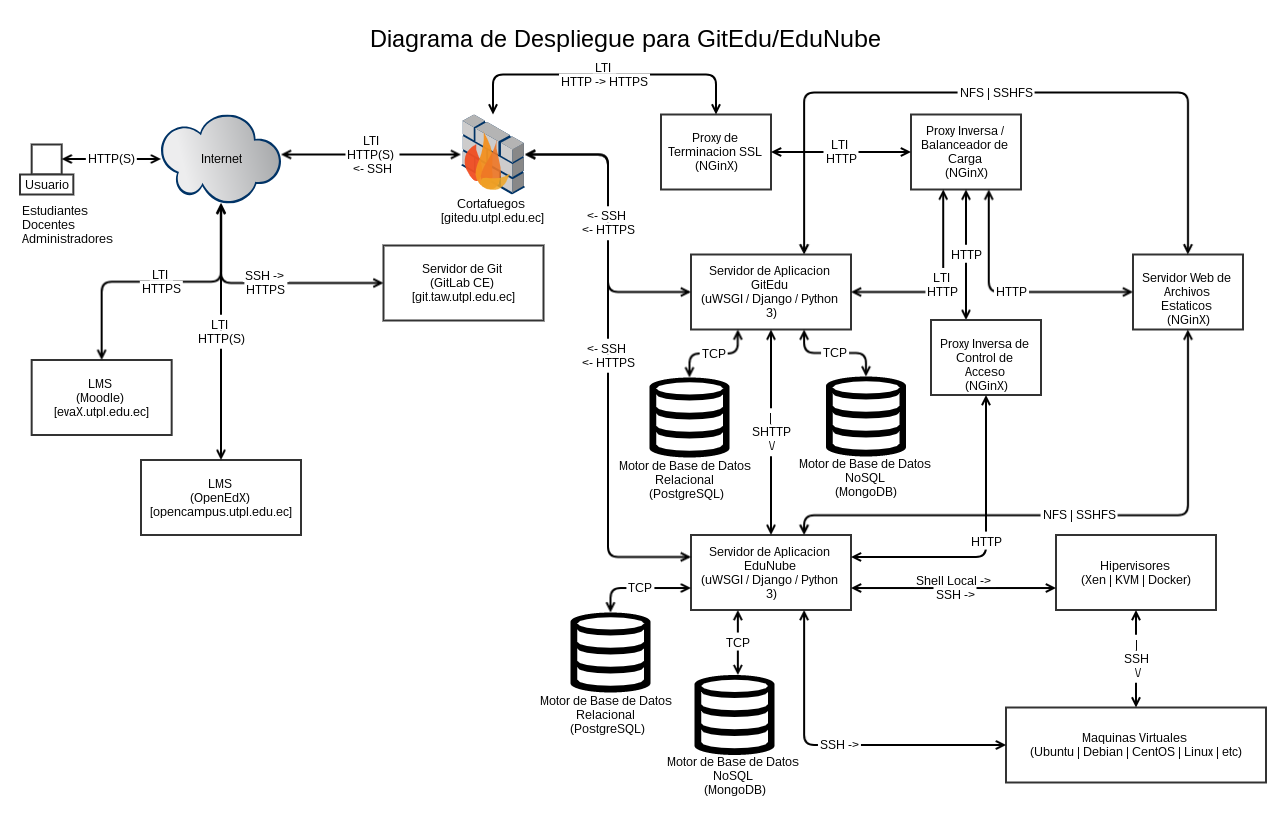
\includegraphics[width=1.4\textwidth]{Figures/desp_ge_en.png}
	  \end{center}
	  \caption{Diagrama de Despliegue para los Sistemas GitEdu y EduNube.}
	  \label{desp_ge_en}
	\end{figure}
\end{landscape}

\subsection{Despliegue}

Como se puede observar en la figura \ref{desp_ge_en}, el despliegue del sistema GitEdu junto al sistema EduNube, consiste en dos redes, una externa que contiene los usuarios finales (Estudiantes, Docentes, Administradores) en adición a sistemas externas como los dos LMS \index{LMS} institucionales (Moodle y OpenEdX) y el servidor de Git (GitLab Community Edition), mientras que la red interna contiene varios componentes que forman el conjunto de sistemas:
\begin{itemize}
	\item \textbf{Cortafuegos}, divide la red interna de la red externa y permite únicamente que pase tráfico HTTP y HTTPS de manera bidireccional (con posibilidad de llamadas LTI \index{LTI} sobre estos protocolos) y la salida de SSH al servidor de Git (para ofrecer mayor seguridad que transferencias sobre HTTP(S)).
    \item \textbf{Proxy de Terminación SSL}, accepta HTTP y HTTPS, pero para asegurar la seguridad de usuarios finales y aplicaciones externas redirecciona al uso del protocolo HTTP a HTTPS. Además descifra conexiones HTTPS entrantes para manejarlos por HTTP dentro de la red interna (reduciendo la carga en otros servidores sin abandonar la seguridad en la red externa) y cifra conexiones salientes. Se utiliza NGinX por su bajo consumo de recursos en comparación con sus competidores como Apache.
    \item \textbf{Proxy Inversa / Balanceador de Carga}, acepta todo el tráfico HTTPS (ahora por el protocolo HTTP dentro de la red interna) entrante y elige en base a la ruta cual servidor se lo puede responder. A futuro este componente permite que se pueda escalar el sistema en lo que permite dividir tráfico entre varios servidores del mismo tipo (por ejemplo dos servidores de aplicación: GitEdu1 y GitEdu2). Se considera que NGinX es la solución más óptima para realizar este rol.
    \item \textbf{Servidor Web de Archivos Estáticos}, se responsabiliza por peticiones de archivos estáticos que no conviene enviar a los servidores de aplicación (quienes los procesaría con mayor lentitud). Estos mismos tienen una conexión NFS o SSHFS con los mismos servidores de aplicación para que estos sean capaces de actualizar remotamente los archivos estáticos en caso de que los mismos cambien (por ejemplo cuando un usuario actualiza su foto de perfil). Estudios de rendimiento demuestran que NGinX cumple este rol de ser servidor web de archivos estáticos mejor que Apache.
    \index{Editar Código} \index{Persistir Código}
    \item \textbf{Servidor de Aplicación ''GitEdu''}, se aloja el sistema GitEdu, desarrollado bajo el marco Django y el lenguaje de programación Python (version 3.x). Se comunica con el servidor externo de Git sobre SSH y dispone tanto de un base de datos relacional como de una no relacional para persistir los distintos tipos de datos que tiene que manejar. Se conecta directamente al Servidor de Aplicación ''EduNube'' mediante SHTTP (HTTP sobre un túnel SSH) utilizando un par de llaves (pública y privada) como esquema de criptografía asimétrica. Se considera uWSGI como mejor servidor de aplicación para el sistema debido a que, a diferencia de su competencia (Gunicorn), esta suporta Websockets.
    \item \textbf{Motores de Base de Datos Relacional}, se alojan datos estructurados para ambos sistemas, tanto GitEdu como NubeEdu.
    \item \textbf{Motores de Base de Datos NoSQL}, se alojan datos no estructurados para ambos sistemas, tanto GitEdu como NubeEdu.
    \item \textbf{Proxy Inversa de Control de Acceso}, restringe acceso al servidor de aplicaciones de EduNube cuando se accede al mismo desde la red externa (a través del proxy inversa).
    \index{Ejecutar Código}
    \item \textbf{Servidor de Aplicación ''EduNube''}, se aloja el sistema EduNube, desarrollado bajo el marco Django y el lenguaje de programación Python (version 3.x). Se comunica con el servidor externo de Git sobre SSH y dispone tanto de un base de datos relacional como una no relacional para persistir los distintos tipos de datos que tiene que manejar. Utiliza un shell local (dentro del mismo servidor) para manejo de un hipervisor local o en el caso de un hipervisor remoto, maneja el mismo sobre SSH. Las máquinas virtuales donde se levanta el hipervisor, también se los controla con SSH. Se considera uWSGI como mejor servidor de aplicación para el sistema debido a que, a diferencia de su competencia (Gunicorn), esta suporta Websockets.
    \item \textbf{Hipervisores}, gestionan máquinas virtuales por parte del sistema EduNube el mismo que envía comandos por SSH o un shell local. A su vez, controla sus máquinas virtuales mediantes SSH. Dentro de las tecnologías de hipervisores se considera Xen, KVM y Docker como buenas opciones para diferentes necesidades. Cada sistema de hipervisores soporta el uso de plantillas para la creación masiva de máquinas virtuales iguales para cada estudiante de una materia.
    \item \textbf{Máquinas Virtuales}, ejecutan código de usuarios y reportan los resultados.
\end{itemize}

\subsubsection{Ventajas de la Arquitectura de Despliegue}
De la misma manera, el diseño de sistemas, subsistemas y módulos en adición al diseño arquitectónico, el diseño de arquitectura de despliegue está orientado a la extensibilidad a través de modularidad, mantenibilidad por la naturaleza de sus capas y módulos, además de escalabilidad y seguridad mantenida a través de mecanismos de aislamiento de componentes que son libres de escalar independientemente entre ellos, la arquitectura de despliegue se orienta a los mismos principios.

La separación de tareas dentro del sistema permite que cada servicio dentro de la arquitectura de despliegue se pueda dedicar a hacer bien su parte correspondiente de la manera más eficiente posible sin responsabilidades que no pueda sostener de forma inadecuada, que es algo importante para empezar a poder garantizar el rendimiento óptimo del sistema. El uso de un cortafuegos y varios proxies inversos al frente de cada sistema también ayuda a aislar los mismos del mundo externo a un nivel de protocolos que reduce las probabilidades de ataques contra los mismos, ofrece seguridad sin sacrificar rendimiento de manera similar al punto anterior de separación de trabajo en roles y asignación al actor más adecuado para el mismo.

Este mismo uso de procesos, especializado cada uno con sus responsabilidades y posible carga de trabajo también sigue ofreciendo escalabilidad a futuro. Esto se realiza con comunicación entre servicios que está sobre protocolos de red para que los mismos puedan estar en un solo recurso (sea servidor físico o virtual) o en varios apartados lo cual permite a futuro la asignación de recursos físicos o virtuales de acuerdo a la necesidad. Esta capacidad para escalar se puede ofrecer gracias al hecho de que los servicios son semi independientes unos de otros, permitiendo n-capas sobre m-niveles físicos/lógicos.

Donde haya dependencias, por ejemplo, sistema de ficheros compartidos para dos capas distintas se puede implementar con protocolos que permitan acceso remoto para las operaciones necesarias, en este caso que los servidores de aplicación sean capaces de actualizar los archivos estáticos en el servidor para este mismo (se lo está considerando esta parte con un NFS o SSHFS). Obviamente en el caso de que estén en el mismo servidor, no se da la necesidad de establecer esta conexión.

En casos donde se necesite mayor seguridad para proteger canales de comunicación, se ha considerado que la mejor forma de controlar esto es con tuneles SSH que encapsulan el tráfico que de por sí solo ocupa un protocolo adecuado. Por ejemplo para consumir el API de EduNube, GitEdu utiliza HTTP sobre SSH (también conocido como SHTTP). De esta forma se puede aprovechar lo que ya existe y que está comprobado como seguro y eficiente (SSH como protocolo, especialmente en su segunda versión, tiene fuertes mecanismos de autenticación y seguridad mientras que al mismo tiempo ofrece menor sacrificio de rendimiento y alta funcionalidad).

A continuación se presenta el alcance del desarrollo, pruebas y despliegue para este trabajo de titulación.

\pagebreak

\begin{landscape}

% figure
\begin{figure}
  \begin{center}
    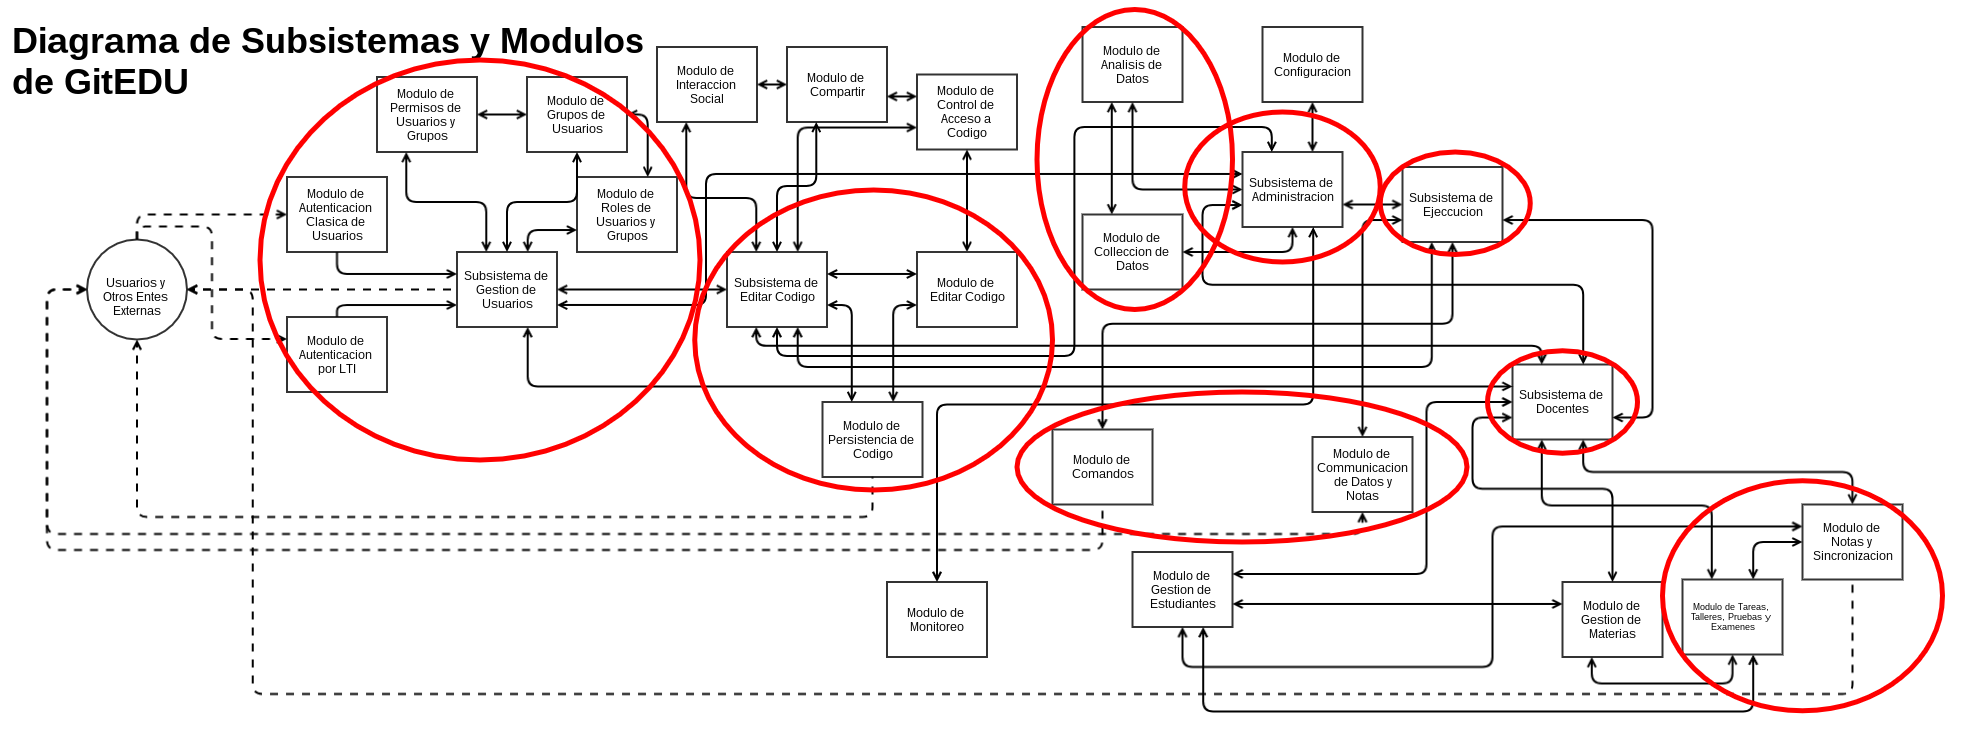
\includegraphics[width=1.7\textwidth]{Figures/alc_mod_ge.png}
  \end{center}
  \caption{Alcance de Módulos para GitEdu.}
  \label{alc_mod_ge}
\end{figure}

\end{landscape}

\subsection{Alcance}

Debido al hecho de que se cuenta con tiempo y recursos limitados para realizar y acabar el trabajo de titulación, se considera un alcance limitado en ciertos aspectos con el fin de terminar con los componentes críticos del sistema dentro del tiempo dado.

Para el sistema GitEdu se considera los siguientes subsistemas y módulos críticos como se puede observar en la figura \ref{alc_mod_ge}:
\begin{itemize}
	\item \textbf{Todo el subsistema de Gestión de Usuarios.} Todos los módulos de este sistema son críticos porque se encargan de cómo los usuarios se autentican y el control de acceso que tiene cada uno. Por lo tanto el subsistema en sí es una parte importante para garantizar seguridad en el sistema final.
    \index{Editar Código}
    \item \textbf{Parte del subsistema de Editar Código.} El subsistema de editar código se considera crítico así como los módulos de editar y de persistir código. El módulo de editar código es crítico porque es la funcionalidad principal de que se trata el sistema mientras que el modulo de persistir codigo viene a ser critico para sincronizar código entre los dos sistemas. No se toma en consideración como críticos los módulos de interacción social, compartir código ni control de acceso a código porque las mismas se tratan de llevar el sistema más allá de su propósito original y son más adecuados para un futuro trabajo.
    \item \textbf{Parte del subsistema de Docentes.} Dentro del subsistema de docentes, se considera crítico elmódulo de crear talleres, pruebas y exámenes en adición a un módulo de notas y su sincronización. Entre estos dos se forma el núcleo de funcionalidad que requieren los docentes dentro de la versión inicial. Dentro de trabajos futuros, se podría extender esta funcionalidad crítica con temas más administrativos como los módulos de gestión de materias y gestión de estudiantes que por el momento no se los considera como funcionalidades críticas para una primera versión estable de este trabajo de titulación.
    \item \textbf{Parte del subsistema de Administración.} Dentro del subsistema de administración, solo se considera que los componentes críticos son la colección de datos y el análisis de los mismos debido a que estos dos módulos respectivamente ayudan en la toma de decisiones que tienen que ver con la escuela de Ciencias de Computación y Electrónica. Los módulos de monitoreo y configuración, aunque podrían ser muy útiles en un ambiente de producción no caen dentro del alcance inicial de esta tesis y por lo tanto no se los considera críticos bajo los parámetros del proyecto. Sin embargo, su implementación podría ser una funcionalidad adicional interesante para un futuro proyecto.
    \index{Ejecutar Código}
    \item \textbf{Todo el subsistema de Ejecución.} Todos los módulos de este sistema son críticos porque se encargan de la comunicación con el sistema EduNube. El módulo de comandos prepara comandos para ejecutar a través del módulo de comunicación de datos y notas se los envía en adición a conseguir resultados y sincronizar notas y calificaciones generadas por EduNube.
\end{itemize}

\begin{landscape}

	% figure
	\begin{figure}
	  \begin{center}
	    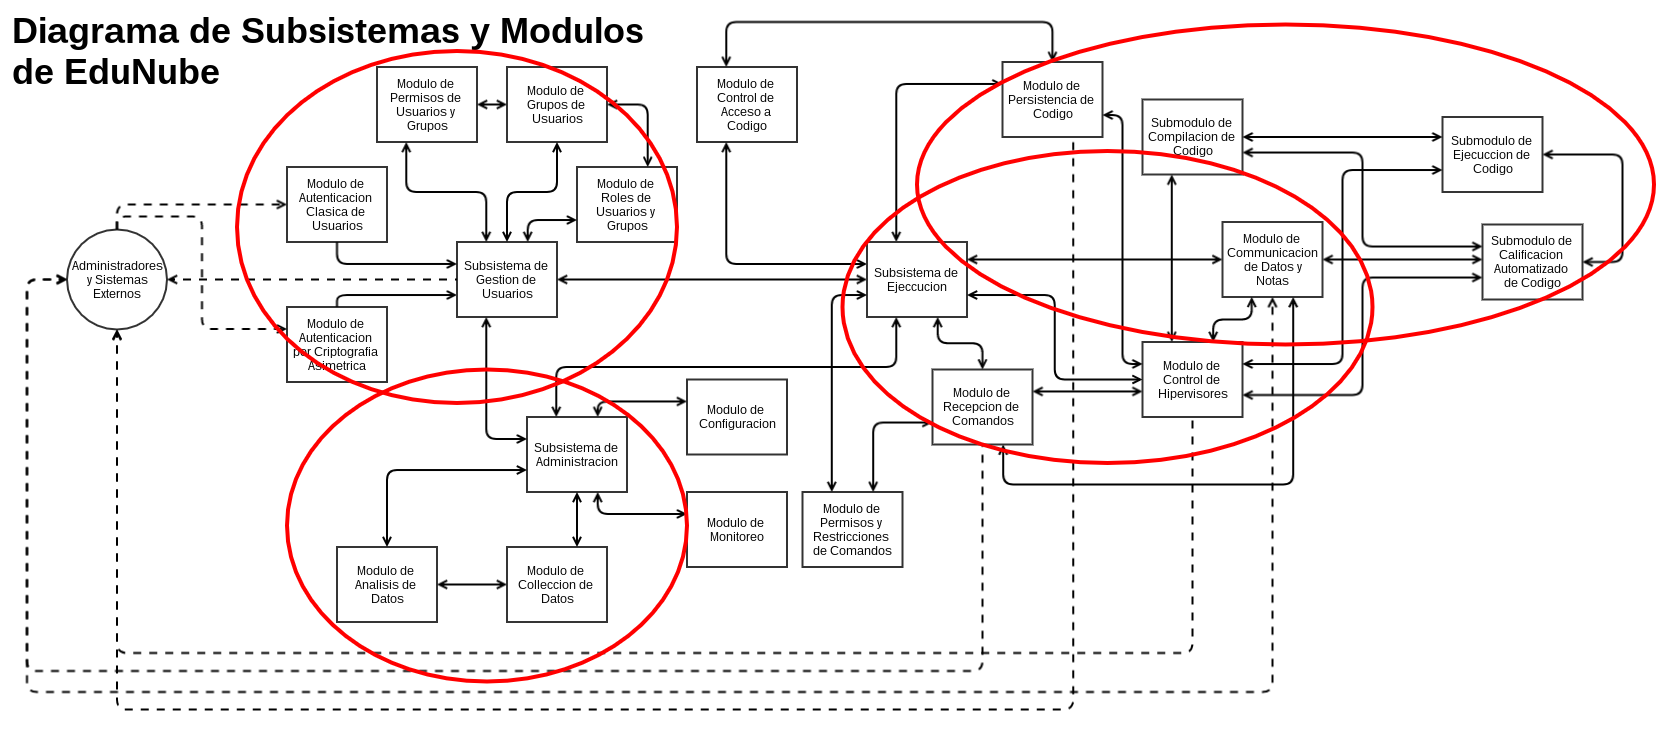
\includegraphics[width=1.7\textwidth]{Figures/alc_mod_en.png}
	  \end{center}
	  \caption{Alcance de Módulos para EduNube.}
	  \label{alc_mod_en}
	\end{figure}

\end{landscape}

Para el sistema EduNube, se considera los siguientes subsistemas y módulos como críticos, como se muestra en la figura \ref{alc_mod_en}:
\begin{itemize}
	\item \textbf{Todo el subsistema de Gestión de Usuarios.} Todos los módulos de este sistema son críticos porque se encargan de cómo los usuarios se autentican contra el mismo sistema y el control de acceso que tienen cada uno en él. Por lo tanto el subsistema en sí es una parte importante para garantizar la seguridad del sistema final.
    \index{Ejecutar Código}
	\item \textbf{Parte del subsistema de Ejecución.} Dentro del subsistema de ejecución se consideran críticos los módulos de comandos (para procesar comandos entrantes), de control de hipervisores (para gestionar recursos virtuales), y de persistencia de código (para recuperar código para su compilación, compilación y ejecución).  Además dentro de los componentes del módulo de control de hipervisores, se considera crítico los submódulos de compilación de código (para aquellos lenguajes que lo requieren), de ejecución (para ejecutar código), y de calificación automatizada de código (para calificar el código de estudiantes). Se considera que los módulos de seguridad adicionales dentro de este subsistema no son necesarios por el momento debido a que el único sistema que tendrá acceso a esta será la de GitEdu. A futuro, donde más sistemas y servicios empiecen a necesitar consumir el API de EduNube, llegará a ser necesario que estos módulos cuenten con seguridad para proveer protección adicional.
	\item \textbf{Parte del subsistema de Administración.} Dentro del subsistema de administración, solo se considera que los componentes críticos se tratan de colección de datos y el análisis de los mismos debido a que estos dos módulos respectivamente ayudan en la toma de decisiones que tienen que ver con la escuela de Ciencias de Computación y Electrónica y el uso del sistema. Los módulos de monitoreo y configuración, aunque podrían ser muy útiles en un ambiente de producción no se involucrab dentro del alcance inicial de esta tesis y por lo tanto no se los considera críticos bajo los parámetros del proyecto. De todas formas su implementación podría ser una funcionalidad adicional e interesante para un futuro proyecto.
\end{itemize}

En cuanto el despliegue (figura \ref{alc_desp_ge_en}), los sistemas externos tomados en consideración para el alcance son Moodle como LMS, y GitLab Community Edition como servidor de control de versiones. En relación a los ambientes virtuales, solo se considera un hipervisor y un sistema operativo para las máquinas virtuales dentro de la versión final (durante el desarrollo se presenta los candidatos, comparación y selección de los mismos). También se incluye dentro del alcance el desarrollo y despliegue de los dos sistemas GitEdu y EduNube con sus respectivas bases de datos utilizando uWSGI como servidor de aplicación. No se incluye dentro del alcance OpenEdX o ningún otro LMS \index{LMS} externo fuera del mencionado previamente, ni las configuraciones del cortafuego y servidores web, estos quedan como responsabilidades institucionales si se desean implementar en el despliegue. Lo que se presenta aquí es una sugerencia del autor basado en su experiencia práctica.

\begin{landscape}

	% figure
	\begin{figure}
	  \begin{center}
	    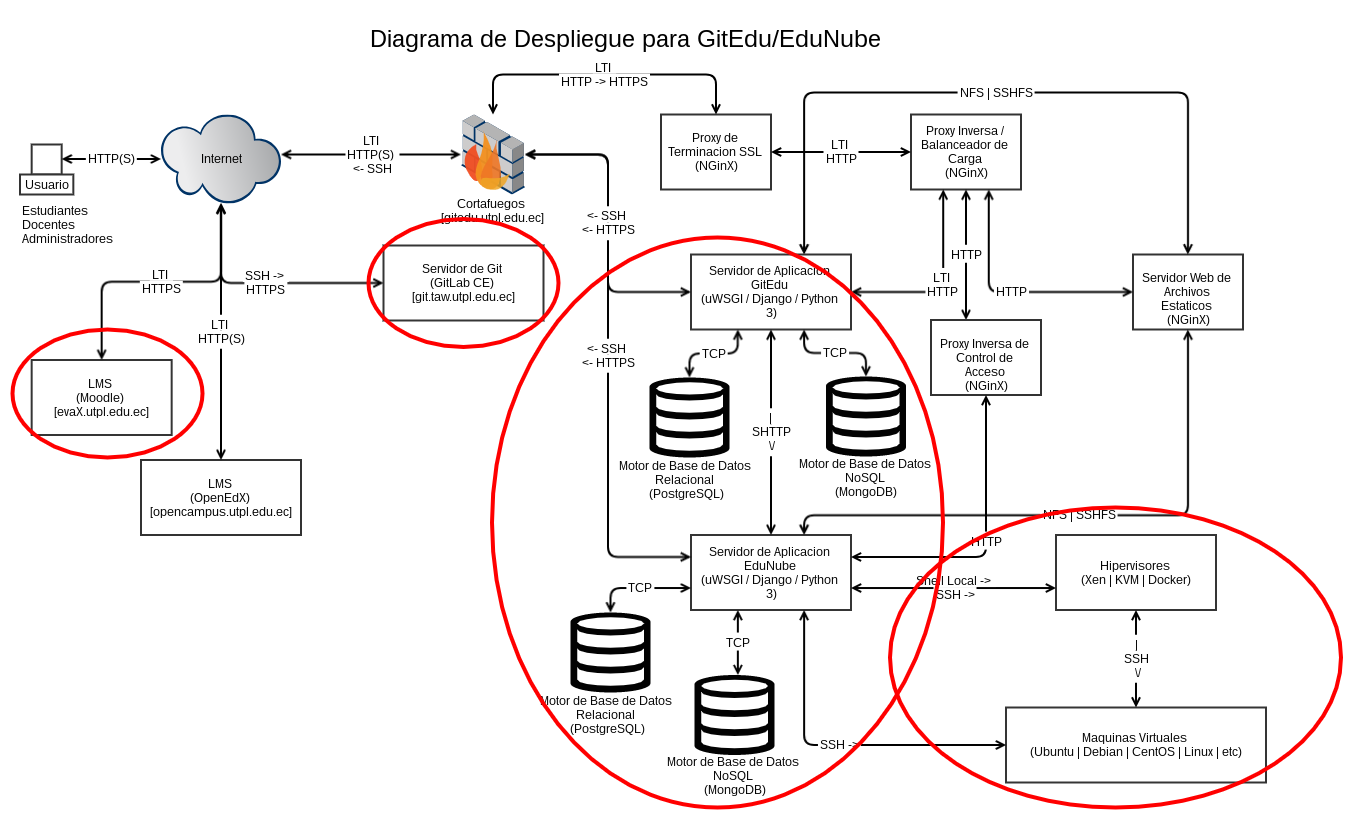
\includegraphics[width=1.4\textwidth]{Figures/alc_desp_ge_en.png}
	  \end{center}
	  \caption{Alcance de Despliegue.}
	  \label{alc_desp_ge_en}
	\end{figure}

\end{landscape}
